\documentclass{scrbook}
\author{Georges de la Porte}
\title{Tractatus Linguisticus}
\usepackage{textcomp}
\usepackage{libertine}
\usepackage{amssymb}
\usepackage[normalem]{ulem}
\usepackage{soul}
\usepackage{subfigure}
\usepackage{tabularx}
\usepackage{booktabs}
\usepackage{multirow}
\usepackage{graphicx}
\usepackage{tikz}
\usepackage[linguistics,edges]{forest}
\usetikzlibrary{positioning} 
\usepackage{langsci-gb4e}
\usepackage{jambox}
\usepackage{langsci-basic}
\usepackage{langsci-optional}
\usepackage{pgfplots}
\usepackage{listings}
\lstset{ %  
  inputencoding=utf8,
  extendedchars=true,
  basicstyle=\ttfamily,        % the size of the fonts that are used for the code  
  literate=%
  {\{}{{{\color{orange}\{}}}1 
  {[}{{{\color{red}[{}}}}1 
  {]}{{{\color{red}]}}}1 
  {)}{{{\color{green})}}}1  
  {(}{{{\color{green}(}}}1  
  {\}}{{{\color{orange}\}}}}1 
} 
 
\usepackage{avm}
\usepackage{setspace} 
\usepackage[framemethod=tikz]{mdframed} 
\usepackage{tipa}
\usepackage{oldprsn}
%  
\input{localhyphenation.tex}
\usepackage[
	natbib=true, 
	style=biblatex-langsci-unified,	citestyle=langsci-authoryear-comp,
% 	style=nature,
	useprefix = true,
	maxbibnames=99,
	uniquename=false,
	mincrossrefs=99,
	maxcitenames=2,
	isbn=false,
	doi=false,
	url=false,
	eprint=false,
        autolang=hyphen,
	backend=biber,
	indexing=cite
]{biblatex}
\addbibresource{mybib.bib}

% \includeonly{%
% chapters/preface,
% chapters/introduction
% }
\begin{document} 
\input{localcommands.tex} 
  
\maketitle                
\frontmatter 

% \currentpdfbookmark{Contents}{name} % adds a PDF bookmark
{\sloppy\tableofcontents}
\include{chapters/preface}
\include{chapters/acknowledgments}
\include{chapters/abbreviations} 
\mainmatter     
 
\chapter{Introduction}\label{sec:intro}
Lorem ipsum dolor sit amet. I first discuss the study in 
Section \ref{sec:study}
The I present the findings in 
Section \ref{sec:findings}
before I conclude in 
Section \ref{sec:conclusion}.

\citet{Chomsky1957}

\section{Study}\label{sec:study}
Pellentesque \textit{sed} egestas \textbf{mauris}. Aliquam \textsc{fermentum} lectus \textit{\textbf{lacus}}, id \textbf{\textsc{feugiat}} leo vi\textsuperscript{verra} vitae. Class aptent\textsubscript{taciti} sociosqu ad litora torquent per conubia nostra, per inceptos himenaeos. Phasellus varius nunc nec turpis aliquam, mollis consequat nisl cursus. Sed eleifend enim nec urna ultrices tincidunt. Maecenas rutrum non enim vel cursus. Praesent non dui tellus. Fusce a lacus et sapien placerat aliquet. Aliquam volutpat pulvinar gravida. Vivamus vitae sodales arcu. 

\subsection{Suspendisse}
Suspendisse tincidunt \large pretium \LARGE magna. \tiny Nam \footnotesize nec ultrices nisl. \scriptsize Nam \itshape augue dui, \normalsize pretium \upshape  sit amet lectus condimentum, mattis\footnote{Or mittas?} blandit risus. Mauris ut nulla eget turpis elementum maximus. Quisque lobortis id orci ac auctor. Proin convallis ante ultrices dapibus tincidunt. Integer\footnote{\label{fn:integer}No real numbers here.} augue libero, mattis sed condimentum eget, facilisis id nisl. In commodo nisi eu purus cursus posuere. Footnote \ref{fn:integer} contains a pun. 

\subsubsection{Maecenas}
Maecenas finibus, 'leo' `quis' "finibus" ``consequat'', nunc quam commodo massa, in malesuada tortor dolor sed urna. 

\begin{quote}
Vivamus ut ornare ipsum, quis hendrerit ligula. Maecenas ac nunc quam. Suspendisse ut tellus vitae orci vulputate volutpat. Etiam tempor leo libero.
\end{quote}

\textonehalf + \textonequarter = \textthreequarters


\textonehalf+\textonequarter=\textthreequarters


\textonehalf~+~\textonequarter~=~\textthreequarters


\textonehalf  +         \textonequarter  =     \textthreequarters


{\textonehalf} + {\textonequarter} = {\textthreequarters}

{\textonehalf}+{\textonequarter}={\textthreequarters}


Pellentesque eget volutpat nisl. Quisque laoreet faucibus ligula, vel porta velit rhoncus a. Integer fermentum enim in dui tincidunt, vitae auctor dolor luctus. Ut imperdiet metus quam, a 

\begin{itemize}
 \item feugiat
 \item ipsum
 \item tempor 
 \item vitae
\end{itemize}

\paragraph{Quisque}
porttitor arcu vel est cursus hendrerit. Proin congue maximus congue. Class aptent 
\begin{enumerate}
 \item taciti sociosqu
 \item  ad litora
 \item torquent per conubia nostra, 
 \item  per inceptos himenaeos. 
\end{enumerate}


Vivamus quis felis pulvinar, ullamcorper mauris ac, porttitor tellus.\\
Proin odio mauris, blandit at pellentesque a, sodales ut nulla.

Nulla nec ultrices lorem, eu elementum urna. Integer vitae ullamcorper risus. 

\noindent
Vestibulum ullamcorper nunc vitae elit commodo varius. Sed nec quam vel quam fringilla sollicitudin.\\
Donec at commodo odio. Aenean et magna massa. Donec elementum sodales leo sit amet efficitur. Maecenas at nunc vehicula, sollicitudin arcu at, suscipit lorem. Vivamus volutpat orci quis felis pulvinar, quis tempor nunc sagittis. Aenean aliquet, nisi eget dignissim mattis, velit sapien lobortis augue, id fermentum lectus ligula vitae diam. Mauris aliquam tortor suscipit ex faucibus, eu elementum urna mattis. 


\paragraph{Donec}
tincidunt ante at dictum tempus.

\begin{itemize}
 \item Vestibulum quis
 \item  ipsum vel nunc 
 \begin{enumerate}
  \item tempor dictum 
  \item eu non tortor. 
  \item[--] Nullam eget massa
  \item  eu eros efficitur ornare.
 \end{enumerate}
 \item  Proin convallis velit eget eleifend consequat.
\end{itemize}
Proin consequat fringilla pretium. Aenean massa tellus, pellentesque eget blandit at, viverra eget turpis. Morbi nisl magna, aliquet id ullamcorper nec, convallis ut neque. Orci varius natoque penatibus et magnis dis parturient montes, nascetur ridiculus mus. Maecenas ut metus mauris. Nulla venenatis, justo eget porta consectetur, diam orci imperdiet elit, vel feugiat dui ipsum sit amet mauris. Donec imperdiet pharetra tellus, ut cursus nunc fermentum eget. Vestibulum elit orci, ultricies in nunc sed, molestie ornare neque. Curabitur a scelerisque ante. Quisque ac auctor elit, et semper metus. Phasellus libero elit, porttitor a odio nec, tempus feugiat leo. Nunc sit amet volutpat felis. 


The circumflex \^{} is used by participants \#2 \& \#3\\
The command {\textbackslash}ref\{\} is used to refer to {\textbackslash}label\{\}s



\subsubsection{Etiam}
 Etiam vestibulum elit a laoreet suscipit. Sed pellentesque quam leo, eget sodales arcu fringilla ut. Maecenas molestie sed ligula at elementum. Praesent tincidunt sapien et ipsum tristique vehicula. In iaculis dolor at nibh fermentum commodo. Etiam condimentum leo at elit ultrices blandit. Suspendisse congue eu leo malesuada sodales. Curabitur cursus libero et leo dictum, a convallis tellus placerat. Etiam commodo massa convallis dolor vestibulum, ut volutpat odio pulvinar. Morbi vitae ipsum posuere, lacinia magna sed, fringilla odio. Praesent molestie commodo est, quis finibus nisi viverra in. Morbi sed ligula porta tellus dapibus feugiat nec ac augue. Quisque rutrum arcu nisl. Duis tincidunt scelerisque fermentum. Donec posuere, felis vel rutrum sagittis, purus nibh eleifend turpis, nec feugiat enim lacus in nisl. 
 
\subsection{Morbi}
Morbi sagittis odio vitae placerat congue. Nunc iaculis imperdiet neque. Integer vulputate euismod ligula in faucibus. Fusce sed lacus vitae turpis malesuada interdum eget non purus. Pellentesque sapien risus, volutpat nec gravida a, pharetra at mauris. Suspendisse rutrum ultrices ipsum eu aliquam. Etiam elementum vehicula metus vitae fermentum. Duis suscipit tellus sapien, at dapibus dui euismod a. Nam in scelerisque orci, facilisis consectetur augue. Maecenas facilisis commodo ipsum. Curabitur ut libero tempus, eleifend diam a, imperdiet enim. Etiam laoreet purus eu nibh pellentesque, non tincidunt quam efficitur. Etiam vel fringilla felis, sed tempus purus. 


\section{Findings}\label{sec:findings}
Aliquam accumsan velit id velit mollis fringilla. Nam sit amet semper orci. Interdum et malesuada fames ac ante ipsum primis in faucibus. In at lectus lorem. Quisque sit amet scelerisque eros. Ut et felis id erat rutrum semper. Duis euismod massa euismod sem dapibus, vel aliquet orci molestie. Praesent eu nibh eget sem hendrerit scelerisque. Ut odio turpis, porttitor sit amet nibh eget, mollis viverra magna. Donec et tellus tortor. Fusce blandit ornare sem non fringilla. Aliquam quis urna ut nisi ultrices imperdiet in facilisis enim. Integer et ipsum sit amet lorem posuere mollis. Vivamus aliquet blandit tempus. 


\subsection{Aenean}
Aenean massa odio, ultrices in lorem in, sollicitudin semper nisl. Aliquam mattis metus id ultricies fringilla. Suspendisse laoreet velit a erat ultricies sollicitudin. Nullam a auctor odio. Nam eu augue mattis, lacinia mauris sed, rutrum leo. Nullam a dolor posuere, iaculis nisl eu, placerat justo. Proin maximus ligula eu arcu eleifend sodales. Phasellus lobortis eleifend varius. Suspendisse potenti. In ac felis id nisi vehicula viverra. 

\subsection{Quisque}
Quisque egestas elementum nunc, non lobortis neque consectetur nec. Suspendisse ac nulla leo. Etiam elementum dolor nec est ultrices, eget ullamcorper ante congue. Phasellus ac blandit purus. Ut sed est commodo, fermentum augue nec, consequat elit. Interdum et malesuada fames ac ante ipsum primis in faucibus. Fusce auctor malesuada enim non posuere. Nullam posuere dignissim mi, sit amet varius lectus porta nec. Praesent cursus mollis mauris nec semper. Phasellus eget odio ipsum. Nam suscipit feugiat ligula, quis porta dolor feugiat et. Vestibulum sit amet massa in augue efficitur semper. Pellentesque lectus lacus, interdum sit amet dapibus non, maximus ut lectus. Sed eget ex eleifend ante aliquet sagittis vitae vel diam. 

\section{Special characters}
áéíóú

àèìòù

šŕŷẅǹĺ̄x

\v s\'r\^y\"w\`n\'l\=x 

ãẽĩõũ

{\'{\~{a}}}
{\'{\~{e}}}
{\'{\~{i}}}
{\'{\~{o}}}
{\'{\~{u}}}

{\~{\'{a}}}
{\~{\'{e}}}
{\~{\'{i}}}
{\~{\'{o}}}
{\~{\'{u}}}

\section{Mathmode}

\noindent
a²+b²=c²\\
$a^2+b^2=c^2$

$x = \frac{-b \pm \sqrt{b^2-4ac}}{2a} $

$$x = \frac{-b \pm \sqrt{b^2-4ac}}{2a} $$

\[x = \frac{-b \pm \sqrt{b^2-4ac}}{2a}\]


\section{New commands}
\newcommand{\PIE}{Proto-Indo-European}
\newcommand{\PP}{Principles \& Parameters}
\newcommand{\chisquare}{$\chi^2$}
\newcommand{\macronacuteo}{\'{\={o}}}
\newcommand{\macronacute}[1]{\'{\={#1}}}

In {\PIE}, the {\PP} were not significant according to the {\chisquare}-test of \macronacuteo{} and \macronacute{x}.

$\aleph \emptyset \neg \infty \surd$

\textinterrobang \textreferencemark \texttildelow $\boxdot\boxminus\boxplus$

\section{Underline}
 \underline{oxo} \underline{ofo} \underline{opo} \underline{o(p)o}\\
 \uline{oxo} \uline{ofo} \uline{opo} \uline{o(p)o}\\
 \ul{oxo} \ul{ofo} \ul{opo} \ul{o(p)o}\\
  
\chapter{Linguistic examples} 

\ea\label{ex:john}
John gives Mary the book
\z

\ea\label{ex:cat}
  \ea The cat is on the mat
  \ex The dog is on the log
  \z
\z

\ea
  \ea[]{\label{ex:mouse1}The mouse is in the house}
  \ex[*]{\label{ex:mouse2}The is in mouse house the}
  \z
\z

While examples \REF{ex:john}, \REF{ex:cat}, and \REF{ex:mouse1} are grammatical, example \REF{ex:mouse2} is not.
 
\ea 
\gll Mi casa es su casa\\
     my house is your house\\
\z

\ea
\gll Ik ben op zoek naar het P.C. Hoofthuis\\
     I  am  on search to the P.C. Hoofthuis\\
\glt `I am looking for the P.C. Hoofthuis.'
\z

\ea
\gll mi-m-iq’-adi-ca            hel deč’\\
\textsc{negvol}-\textsc{m}-do:\textsc{ipfv}-\textsc{proh}-\textsc{ptcl} this  song  \\
\glt   ‘Don’t sing this song!’
\z

\ea
Tên{\dots} khátpy ra khuthun tho mo nhy ndo khá than jáwi arak anhi khãm mbaj to no.\\
\gll   tên           khátpy=ra   khu-thu=n  t<h>o   mo=nhy   ndo khá  tha=n              jáwi        arak    anhi khãm ∅-mba-j             to   no    \\
      unexpectedly monster=\textsc{nom} 3-load.on.back=\&.\textsc{ss} <3>with go.\textsc{pl}=\&.\textsc{ds} eye skin rupture=\&.\textsc{ss} as.they.say already self in   3-hear-\textsc{nmlz} with lie.down.\textsc{sg}\\
\glt ‘Unexpectedly, the \textit{khátpy} monster had loaded it (the basket) on his back and was carrying it, and he (the ancestor) woke up and was already lying down listening.’
\z

    
\ea
\gllll La reina de Inglaterra se llama Isabel      \\
       La regina d' Inghilterra si chiama Elisabetta\\
       La reine d' Angleterre s' appelle Élisabeth   \\
       The queen of England \textsc{refl} call Elizabeth    \\
\glt  ‘The queen of England is called Elizabeth'
\z

\begin{exe}
\exr{ex:john} John gives Mary the book  
\end{exe}

\ea\label{ex:john2}
\gll John gives Mary the book \\
     A   ~      R     ~  T \\
\z

\begin{exe}
\exp{ex:john2}
\gll John gives the book to  Mary \\
     A   ~       ~  T ~ R \\
\end{exe}


\ea 
  \ea {Ik ga het huis uit.}\jambox{(Dutch)}
  \ex {Ich gehe aus dem Haus.}\jambox{(German)}
  \ex {I leave the house.}\jambox{(English)}
  \z
\z
 
 
\section{Trees}  
 
\begin{forest}
[S [NP] [VP]]
\end{forest}

\begin{forest}
[S 
  [NP [The] [girl]] 
  [VP 
    [V [eats]] 
    [NP [the super-tasty chocolate pudding she bought at the festival, roof]]
  ]
]
\end{forest}

\begin{forest}
[S 
  [NP [The lady,roof]]
  [VP 
    [V [sees] ]
    [NP [the monkey, roof]]
    [PP [with the telescope, roof]]
  ]
]
\end{forest}

\begin{forest}
[S 
  [NP [The lady,roof]]
  [VP 
    [V [sees]]
    [NP 
      [the] 
      [N$'$ [N [monkey]] 
	[PP [with the telescope, roof]]
      ]
    ]
  ]
]
\end{forest}

 \begin{forest} for tree={grow'=east,delay={where content={}{shape=coordinate}{}}}, for descendants={anchor=west, child anchor=west}, forked edges, l sep=2em
  [Proto-Basa
    [
      [Basa-Kontagora]
      [Basa-Gumna]
    ]
    [Koromba]
    [
      [Basa-Gurara]
      [Basa-Kwali]
    ]
    [
      [Basa-Benue]
      [Basa-Makurdi]
    ]
  ]  
 \end{forest} 
 
 \begin{forest} baseline, where n children=0{tier=word}{} ,for tree={align=center,base=bottom}
 [ω
    [ω$_w$
      [Σ
        [σ$_s$\\bun]
        [σ$_w$\\des]
      ]]
    [ω$_s$
      [ω$_s$
        [ω$_s$
           [ω$_s$
              [Σ
                [σ\\ar]
              ]]
           [ω$_w$
              [Σ
                [σ\\beits]
              ]]]
          [ω$_w$
              [Σ
                [σ\\amts]
              ]]]
          [ω$_w$
              [Σ$_w$
                [σ$_s$\\prä]
                [σ$_w$\\si]
              ]
              [Σ$_s$
                [σ\\dent]
              ]]]
]
\end{forest}
 
 
\begin{forest}
[CP
  [DP,name=tgt]
    [IP
      [,phantom]
      [VP
	[DP]
	[V$’$ 
	  [V] 
	  [\sout{DP},name=src]
      ]
    ]
  ]
]
\draw[->] (src) to[out=south west,in=south] (tgt);
\end{forest}

 
\section{Non-Latin scripts}
- Write "Happy New Year" in Russian, Greek, Chinese 

С новым годом

Ευτυχισμένο το νέο έτος

\newfontfamily\cn[Mapping=tex-text,Ligatures=Common,Scale=MatchUppercase]{AR PL UMing CN}
\newcommand{\zh}[1]{{\cn #1}} 
{\cn 新年快乐}


- Write \textit{LOTschool, UVA, Amsterdam} in IPA\\{}
[\textipa{"lO\|[t sxo:l, "y:fa:, Amst@r"\|[dAm}]\\{}
[\textipa{"lOt sku:l, "u:fa, "\ae mst5d\ae m}]

----

 
\chapter{Images} 
Sed blandit sem velit, sed iaculis lectus elementum at. Morbi posuere nibh erat, et aliquam urna dictum sed. Quisque fringilla magna turpis, ut sodales nulla rhoncus non. Donec id lacus velit. Praesent tempus, nibh sed consectetur vulputate, libero ante interdum leo, eu ultrices sapien sapien id dui. Phasellus et rutrum elit. Cras quis quam vitae urna ultrices bibendum vel eget turpis. Ut ultrices ut est sed efficitur. Morbi neque ante, dictum ac diam vel, cursus suscipit nunc. Suspendisse sagittis ut nisl quis hendrerit. Praesent vulputate ac augue eu pretium. Mauris at sollicitudin elit. Suspendisse in interdum ex.

\includegraphics{akkadian.png}

   
   Suspendisse diam lectus, laoreet eu maximus eget, sollicitudin et dolor. Phasellus imperdiet elit et arcu porta iaculis. Suspendisse tempor purus nec porta accumsan. Ut tempus augue quam, vitae rhoncus velit hendrerit aliquam. Fusce ac turpis id sem feugiat placerat. Nunc nec ullamcorper nibh, in feugiat lectus. Fusce ut nisl bibendum, tincidunt magna vitae, scelerisque metus. In nec dui vestibulum ante dapibus tempus. Curabitur vel purus rutrum, dictum lectus a, interdum tellus. Etiam hendrerit ante sem, a sodales urna finibus a. Vestibulum ante ipsum primis in faucibus orci luctus et ultrices posuere cubilia Curae; Vivamus posuere nec nibh in gravida. Ut mattis condimentum imperdiet. Vivamus tempus viverra diam quis dictum. Donec nulla mi, facilisis eget sapien eu, tristique malesuada purus. 
   
\includegraphics{akkadian.png}

Pellentesque egestas, sem quis elementum gravida, ex diam interdum orci, id venenatis justo dolor eget risus. Vestibulum blandit ante et feugiat feugiat. Suspendisse potenti. Sed a sollicitudin enim, nec porttitor felis. Vestibulum sed justo vehicula, ultrices arcu nec, hendrerit lacus. Aenean luctus ipsum sit amet enim sodales placerat sit amet et dolor. In turpis ex, scelerisque in maximus ut, placerat ullamcorper ex. Cras in blandit enim. 
\includegraphics{tablet.jpg}


Maecenas et suscipit mauris. Aliquam laoreet, ligula sed ultrices tristique, dolor nisl elementum nisi, sit amet sagittis sapien lacus sed metus. Sed ipsum ligula, consequat ut erat eget, vehicula ultrices purus. Aenean aliquam eu nunc et ultricies. Ut tincidunt mattis ipsum, hendrerit venenatis ipsum sollicitudin eu. Proin egestas purus et elementum posuere. Nunc tempus maximus felis id posuere. Suspendisse scelerisque mauris vitae ligula venenatis, vel fermentum magna laoreet. Ut hendrerit felis dolor, ac cursus nunc commodo vitae.


\begin{figure} 
\includegraphics{akkadian.png}
\caption{Akkadian script}
\label{fig:akkadianscript}
\end{figure}


\begin{figure} 
\includegraphics[width=\textwidth]{akkadian.png}
\caption{Akkadian script scaled to text width}
\label{fig:akkadianscript}
\end{figure}


\begin{figure} 
\includegraphics[height=.3\textheight]{akkadian.png}
\caption{Akkadian script scaled to 30\% of text height}
\label{fig:akkadianscript}
\end{figure}


Sed pretium sem sit amet arcu fermentum, sed fringilla nunc volutpat. Nulla tempor pretium viverra. Donec ut justo non risus tempus aliquam quis vitae lectus. Sed ornare viverra tellus et rutrum. In maximus risus in rhoncus rhoncus. Nulla id risus dui. Ut a felis id arcu accumsan ornare eget id erat. Sed ex arcu, dignissim at justo in, finibus aliquet dolor. Mauris sapien mi, faucibus sit amet justo ac, rutrum rutrum turpis. Etiam a nibh eu purus tempor egestas a nec quam. Nunc diam massa, semper a urna eu, placerat semper eros. Maecenas auctor hendrerit nibh quis finibus. 
Akkadian script is illustrated in Figure \ref{fig:akkadianscript}


\begin{figure} 
\includegraphics[height=5cm]{akkadian.png}~
\includegraphics[height=5cm]{tablet.jpg}

\caption{Akkadian script and tablets}
\end{figure}



Mauris metus nisl, egestas at blandit sit amet, suscipit id metus. Phasellus hendrerit, lacus nec ultrices ullamcorper, leo elit egestas ligula, in auctor sapien purus eu massa. Maecenas at maximus sapien, eget tempor metus. Nullam lacinia lectus quis erat tristique, a ornare libero dignissim. Etiam diam tortor, tristique at consectetur et, dignissim ac nulla. Sed vehicula, libero id faucibus ultrices, ante dui mattis massa, vitae porttitor libero elit cursus erat. Mauris sit amet dictum ex. Nulla in tellus ac enim vulputate sollicitudin id at lectus. Vestibulum interdum sit amet tortor vel egestas. Pellentesque lacus nibh, venenatis nec pulvinar ac, viverra eu lacus. Integer id leo in enim elementum faucibus. 

\begin{figure}
\centering
\subfigure[Akkadian writing system]{\includegraphics[width=.4\textwidth]{akkadian.png}}
~
\subfigure[Clay tablets]{\includegraphics[width=.4\textwidth]{tablet.jpg}}
\caption{Figure with subfigures}
\end{figure}


 Nullam gravida id magna eget rhoncus. Proin ullamcorper lacinia lacus, eu consequat diam fermentum condimentum. Nulla augue ante, semper non accumsan a, mattis eu mi. Donec viverra enim lacus, ut volutpat quam lobortis a. Sed in nunc ac orci elementum pellentesque. Nunc posuere enim est, et bibendum neque facilisis ac. Praesent accumsan massa sed neque porttitor accumsan. Donec lacinia ac urna at faucibus. Aliquam gravida feugiat metus vitae malesuada. In porta ligula orci, et mollis dui vehicula ac. Lorem ipsum dolor sit amet, consectetur adipiscing elit. Nam eu lobortis dui. Praesent tellus urna, tempor a elit nec, cursus sagittis velit. Etiam dapibus vel felis eu hendrerit. In eleifend, lectus in gravida iaculis, urna metus porttitor metus, a condimentum neque magna a nibh.
 
 

 
\chapter{Tables}
\begin{tabular}{llll}
 1&2&3&4\\
 5&6&7&8\\
 9&10&11&12\\
 13&14&15&16
\end{tabular}

Vestibulum turpis lectus, vulputate id lobortis et, mattis ut turpis. Etiam nisi odio, semper vel commodo at, lacinia sed mauris. Vivamus at blandit risus, eu tristique eros. Morbi venenatis ligula eu consectetur pulvinar. In eget lectus lacinia, vehicula magna in, dapibus dui. Suspendisse potenti. Vestibulum ante ipsum primis in faucibus orci luctus et ultrices posuere cubilia Curae; Phasellus facilisis finibus purus quis sagittis.

\begin{tabular}{ccrr}
 1&2&3&4\\
 5&6&7&8\\
 9&10&11&12\\
 13&14&15&16
\end{tabular}

Duis pharetra erat id sapien venenatis, id maximus quam mattis. Curabitur tincidunt eros quis lectus scelerisque tincidunt. Curabitur turpis elit, maximus tempor sagittis in, semper et nunc. Ut rhoncus viverra dui, eget gravida orci maximus sit amet. Donec vulputate nunc nulla, rhoncus tempor nisl laoreet eu. Ut fermentum laoreet velit, a auctor quam consequat et. Etiam sit amet ante fringilla, rhoncus nisi eget, varius est. Nullam id ultrices urna. Cras elit urna, condimentum in ante sed, ullamcorper pharetra mauris. Nullam sollicitudin magna et nunc gravida porta. 

\begin{tabular}{p{5cm}rcl}
 1&2&3&4\\
 5&6&7&8\\
 9&10&11&12\\
 13&14&15&16
\end{tabular}

\begin{table}
\begin{tabular}{p{2cm}rp{2cm}l}
 1&2&3&4\\
 5&6&7&8\\
 9&10&11&12\\
 13&14&15&16
\end{tabular}
\caption{Tabular in table with caption}
\label{tab:intro}
\end{table}

Table \ref{tab:intro} has a caption.


\begin{table}
\begin{tabularx}{\textwidth}{XXXX}
 1&2&3&4\\
 5&6&7&8\\
 9&10&11&12\\
 13&14&15&16
\end{tabularx}
\caption{Tabularx}
\label{tab:tabularx}
\end{table}

Table \ref{tab:tabularx} has the width of the page

\begin{table}
\begin{tabularx}{.66\textwidth}{XXXX}
 1&2&3&4\\
 5&6&7&8\\
 9&10&11&12\\
 13&14&15&16
\end{tabularx}
\caption{Tabularx at .66 width}
\label{tab:tabularx66}
\end{table}

Table \ref{tab:tabularx66} has .66 of the width of the page



\begin{table}
\begin{tabularx}{\textwidth}{XXXX}
\toprule
 1&2&3&4\\
 \midrule 
 5&6&7&8\\
 9&10&11&12\\
 13&14&15&16\\
 \bottomrule
\end{tabularx}
\caption{Tabularx with lines}
\label{tab:tabularxrules}
\end{table}

Table \ref{tab:tabularx66} has lines



\begin{table}
\begin{tabularx}{\textwidth}{XXXX}
\hline
 1&2&3&4\\
\hline
 5&6&7&8\\
\hline
 9&10&11&12\\
\hline
 13&14&15&16\\
 \hline
\end{tabularx}
\caption{Tabular with many lines}
\label{tab:tabularxhline}
\end{table}



\begin{table}
\begin{tabularx}{\textwidth}{|X|X|X|X|}
\hline
 1&2&3&4\\
\hline
 5&\multicolumn{2}{c|}{6.5}&8\\
\hline
 9&10&11&12\\
\hline
 13&14&15&16\\
 \hline
\end{tabularx}
\caption{Tabular with horizontally merged cell}
\label{tab:tabularxmulticolumns}
\end{table}


\begin{table}
\begin{tabularx}{\textwidth}{|X|X|X|X|}
\hline
 1&2&3&4\\
\hline
 5&\multirow{2}{*}{8}& 7 &8\\
\cline{1-1}\cline{3-4}
 9& &11&12\\
\hline
 13&14&15&16\\
 \hline
\end{tabularx}
\caption{Tabular with vertically merged cell}
\label{tab:tabularxmultirow}
\end{table}
 
 
\include{chapters/codesnippets} 
\chapter{Conversation analysis}
\mdfdefinestyle{firstfoc}{linecolor=white,backgroundcolor=gray!10!white,innerleftmargin=0.01mm,innertopmargin=0.01mm}  
\mdfdefinestyle{secondfoc}{linecolor=white,backgroundcolor=gray!30!white,innerleftmargin=0.01mm,innertopmargin=0.01mm} 
 \mdfdefinestyle{thirdfoc}{linecolor=white,backgroundcolor=gray!50!white,innerleftmargin=0.01mm,innertopmargin=0.01mm}
 
\newcommand{\transheader}[2]{\ea\label{#1}#2\z\vspace*{-.7\baselineskip}}

\newlength{\transindent}
\setlength{\transindent}{2mm}

\newenvironment{transbox}[3][\footnotesize]{%
  \setstretch{0.7}
  \medskip\noindent
  \hspace*{\transindent}% 
  #1
  \parbox[b]{3mm}{#1  \oldstylenums{#2}\vphantom{fj}}%
  \parbox[b]{8mm}{#1\scshape  \MakeLowercase{#3} \vphantom{fj}}%
  \begin{minipage}[t]{11cm}#1\vspace*{-1.9\baselineskip}{}\,\vphantom{fj}}
  {\end{minipage}}

\newcommand{\emptytransbox}[3][\footnotesize]{%
  \medskip\noindent
  \hspace*{\transindent}% 
  \parbox{3mm}{#1 \oldstylenums{#2}}%
  \parbox{8mm}{~}%
  #1 #3\\
}

\newcommand{\xtransbox}[4][\footnotesize]{%
  \medskip\noindent
  \hspace*{\transindent}% 
  \parbox{3mm}{#1 \oldstylenums{#2}}%
  \parbox{8mm}{\scshape #1 #3}%
  #1 #4
}


\ea
\begin{lstlisting}
JA: Where did you put the bloody papers? 
CI:                       I did not put them ANYWHERE!
\end{lstlisting}
\z

\ea 
\begin{transbox}{1}{Kar}
\begin{verbatim}
Ay kuraka djiwa karrimbuk[tharr.
Ay kura    -ka  djiwa karrim            -buktharr
Oh NC:WATER-TOP that  3SG.S.stand(3)NFUT-be_red
\end{verbatim}\vspace*{-3mm}
Ay that tea is too strong ((too red)).
\end{transbox}

\begin{transbox}{2}{Ali}
\begin{verbatim}
                         [Yawu munak [kura path- pathayu]=
                          yawu munak  kura     STRI patha=yu
                          hey  sister NC:WATER STRI good =CL
\end{verbatim}\vspace*{-3mm}
Hey sis, fresh water,
\end{transbox}

\begin{transbox}{3}{Ali}
\begin{verbatim}
                                     [((points to car))]
\end{verbatim}\vspace*{-3mm}
\end{transbox}
\z


 
\chapter{Functional Discourse Grammar representations}
\ea
(Π M$_1$: [\\
~~~~~~~~(Π A$_1$: [\\
~~~~~~~~~~~~~~~~(Π F$_1$: ILL (F$_1$): Σ (F$_1$))$_\Phi$\\
~~~~~~~~~~~~~~~~(Π P$_1$: {\dots} (P$_1$): Σ (P$_1$))$_\Phi$\\
~~~~~~~~~~~~~~~~(Π P$_2$: {\dots} (P$_2$): Σ (P$_2$))$_\Phi$\\
~~~~~~~~~~~~~~~~(Π C$_1$ : [\\
~~~~~~~~~~~~~~~~~~~~~~~~~~~~~~~~(Π TI [{\dots}] (TI): Σ (TI))$_\Phi$\\
~~~~~~~~~~~~~~~~~~~~~~~~~~~~~~~~(Π RI [{\dots}] (RI): Σ (RI))$_\Phi$\\
~~~~~~~~~~~~~~~~](C$_1$): Σ (C$_1$))$_\Phi$\\
~~~~~~~~](A$_1$): Σ (A$_1$))$_\Phi$\\
](M$_1$): Σ (M$_1$))$_\Phi$ \\
\z

----

 
\include{chapters/newenvironments} 
\chapter{Drawings}
\definecolor{lsRichGreen}{cmyk}{0.6,0,0.9,0.35}
 

\eabox{
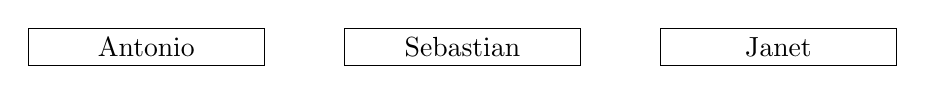
\begin{tikzpicture}
 \node[rectangle,draw,minimum width = 3cm] (s) {Sebastian};
 \node[rectangle,draw,minimum width = 3cm, left = 1cm of  s] (a) {Antonio};
 \node[rectangle,draw,minimum width = 3cm, right = 1cm of  s] (j) {Janet};
\end{tikzpicture}

}


\eabox{ 
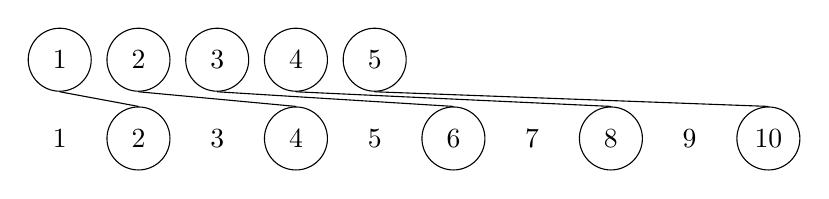
\begin{tikzpicture} 
\node[draw,minimum width = 8mm, circle] (A) {1};
\node[draw,minimum width = 8mm,circle, right of=A] (B) {2};
\node[draw,minimum width = 8mm,circle, right of=B] (C) {3};
\node[draw,minimum width = 8mm,circle, right of=C] (D) {4};
\node[draw,minimum width = 8mm,circle, right of=D] (E) {5};


\node[minimum width = 8mm, below of=A] (a) {1};
\node[draw,minimum width = 8mm,circle, right of=a] (b) {2};
\node[minimum width = 8mm, right of=b] (c) {3};
\node[draw,minimum width = 8mm,circle, right of=c] (d) {4};
\node[minimum width = 8mm, right of=d] (e) {5};
\node[draw,minimum width = 8mm,circle, right of=e] (f) {6};
\node[minimum width = 8mm, right of=f] (g) {7};
\node[draw,minimum width = 8mm,circle, right of=g] (h) {8};
\node[minimum width = 8mm, right of=h] (i) {9};
\node[draw,minimum width = 8mm,circle, right of=i] (j) {10};

\draw(A.south)--(b.north);
\draw(B.south)--(d.north);
\draw(C.south)--(f.north);
\draw(D.south)--(h.north);
\draw(E.south)--(j.north);

\end{tikzpicture}
}

\eabox{
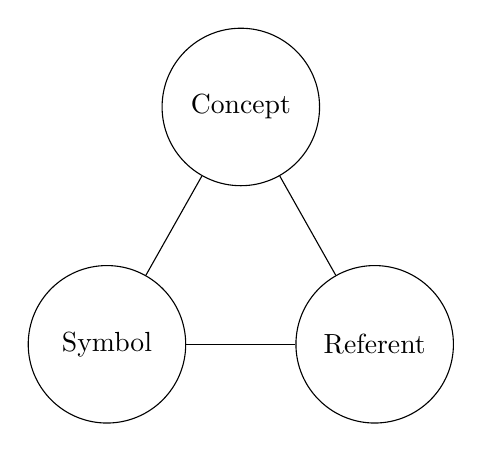
\begin{tikzpicture} 
\node[circle,draw,minimum width=2cm] (c) {Concept};
\node[circle,draw,minimum width=2cm,below=1cm of c,xshift = -1.7cm] (s) {Symbol};
\node[circle,draw,minimum width=2cm,below=1cm of c,xshift =  1.7cm] (r) {Referent};

\draw(s) -- (r);
\draw(s) -- (c);
\draw(c) -- (r);
\end{tikzpicture}
}

 
\eabox{
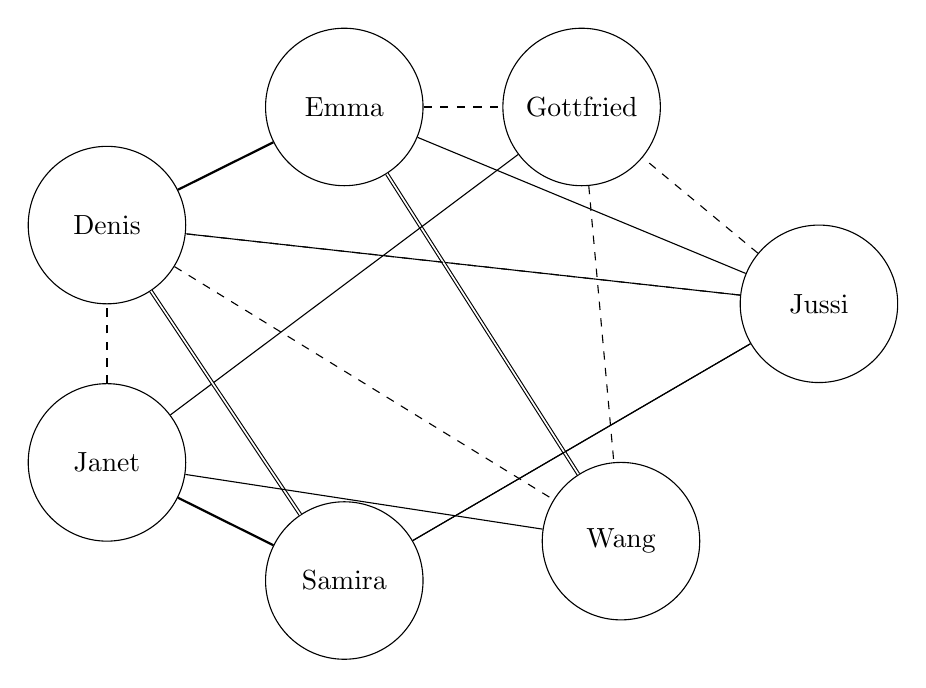
\begin{tikzpicture} 
\node[circle,draw,minimum width=2cm] (e) {Emma};
\node[circle,draw,minimum width=2cm,left =  1cm  of e, yshift=-15mm] (d) {Denis};
\node[circle,draw,minimum width=2cm,below =  1cm  of d] (j) {Janet};
\node[circle,draw,minimum width=2cm,right =  1cm  of j, yshift=-15mm] (s) {Samira};
\node[circle,draw,minimum width=2cm,right = 1cm  of e] (g) {Gottfried};
\node[circle,draw,minimum width=2cm,right = 1cm  of g, yshift=-25mm] (y) {Jussi};
\node[circle,draw,minimum width=2cm,right = 1.5cm of s, yshift=  5mm ] (w) {Wang};

\draw[dashed](e) -- (g);
\draw[thick](j) -- (s);
\draw(d) -- (y);
\draw[dashed](d) -- (w);
\draw[thick](d) -- (e);
\draw(s) -- (y);
\draw[dashed](y) -- (g);
\draw[double](w) -- (e);
\draw(g) -- (j);
\draw[dashed](g) -- (w);
\draw(e) -- (y);
\draw[double](d) -- (s);
\draw[dashed](j) -- (d);
\draw(w) -- (j);
\draw[dashed](y) -- (d);
\draw(y) -- (s);
\end{tikzpicture}
}


 
\chapter{Plots and charts}
\begin{figure}
\centering 
  \barplot{level}{\%}{non-existent,A1,A2,B1,B2,C1,C2,NS/NSE}{
    (non-existent,2)
    (A1,6)
    (A2,11)
    (B1,49)
    (B2,54)
    (C1,21)
    (C2,7)
    (NS/NSE,4)
  }  
  \caption{A bar chart}
\end{figure}

\begin{figure}
\centering
  \begin{tikzpicture}
    \begin{axis}[
	xlabel={Proficiency level},  
	ylabel={VOT (ms)}, 
	axis lines*=left, 
	width  = .7\textwidth,
	height = .3\textheight,
	nodes near coords, 
	xtick=data,
	x tick label style={},  
	ymin=0,
	ybar,
	bar width=10mm,
	enlarge x limits=0.25,
	symbolic x coords={NES, Low level, High level},
	legend style={at={(1,0.4)},anchor=west}
	]
	\addplot+[ybar,blue!80!black,fill=blue!50!black] plot coordinates {
	    (NES, 65.47 ) (Low level,  43.27) (High level,60.11 )
	}; 
	\addplot+[ybar,green!80!black,fill=green!50!black] plot coordinates {
	    (NES,65.47 ) (Low level, 47.87) (High level,55.83)
	}; 
	\legend{T1, T2}
    \end{axis} 
  \end{tikzpicture} 
  \caption{Grouped bar chart}  
\end{figure}

\begin{figure}
\centering
  \begin{tikzpicture}
    \begin{axis}[
	width  = .5\textwidth,
	height = .6\textheight,
	ylabel={},
	xlabel={}, 
	symbolic y coords={
	  Lack of content organization,
	  Lack of thematic content, 
	  Speaker's storytelling ability, 
	  Vocabulary, 
	  Grammar,
	  Number of silent pauses,  
	  Repetition of words,
	  Intonation, 
	  Rhythm, 
	  Word stress, 
	  Pronunciation of vowels and consonants 
	},   
	ytick=data,
	axis lines*=left,  
	xmin=0,
	xbar,
	bar width = 5mm,
	nodes near coords,
	nodes near coords align={horizontal},
	axis on top, 
    ]    
    \addplot+[green!80!black,fill=green!60!black] coordinates {%
    (10,Word stress) 
    (9,Rhythm) 
    (11,Pronunciation of vowels and consonants) 
    (9,Intonation) 
    (2,Grammar) 
    (2,Vocabulary)
    (2,Repetition of words)  
    (2,Number of silent pauses)
    (2,Speaker's storytelling ability) 
    (2,Lack of thematic content) 
    (1,Lack of content organization) 
    }; 
    \end{axis}
  \end{tikzpicture} 
  \caption{Horizontal bar chart}
\end{figure}


  
 
\chapter{AVMs}

\ea\label{ex:showcases:avm-complicated} 
  \begin{avm}
    {\itshape word\/} $\rightarrow$
    \[ morphs & $\@{e_1}\bigcirc\cdots\bigcirc\@{e_n}$\\
       morsyn & \@0 $(\@{m_1}\uplus\cdots\uplus\@{m_n})$\\
       rules  & \< \[ morphs & \@{e_1}\\
                      mud & \@{m_1}\\ 
                      morsyn & \@0\], \ldots ,
                    \[morphs & \@{e_n}\\
                      mud    & \@{m_n}\\ 
                      morsyn & \@0\] \>
    \]
  \end{avm}
\z 
   
\sloppy
\printbibliography
\end{document}  